\documentclass{article}
\usepackage{graphicx}
\usepackage{fullpage}
\title{Implementation of the exponential function}
\author{Morten Engsvang}
\date{}
\begin{document}
\maketitle
\begin{abstract}
I will briefly introduce the mathematical background for the exponential function before I introduce and discuss the 'quick and dirty' implementation given in the exercise.\\
In the end I also plot the implementation alongside the one given in the mathematical library.
\end{abstract}

\section{The exponentialfunction}
The exponential function in itself is defined as follows with the derivative given:
\begin{equation}
	f(x)=ab^x,\frac{d}{dx}ab^x = a\cdot log_e(b)b^x
\end{equation}
The function usually denoted the exponential function is the natural exponential function where $b=e$,which then has the property that it is its own derivative.

\section{The quick and dirty implementation}
A C-function, ex(x), is given in the exercise which can be described as follows:\\
If the function value is less than 0 it will return $\frac{1}{ex(-x)}$. If $x>1./8$ it will return pow(ex(x/2),2). Finally if it passes these checks it will return the following:
\begin{equation}
	1+x\cdot\left(1+\frac{x}{2}\cdot\left(1+\frac{x}{3}\cdot\left(1+\frac{x}{4}\cdot\left(1+\frac{x}{5}\cdot\left(1+\frac{x}{6}\cdot\left(1+\frac{x}{7}\cdot\left(1+\frac{x}{8}\cdot\left(1+\frac{x}{9}\cdot\left(1+\frac{x}{10}\right)\right)\right)\right)\right)\right)\right)\right)\right)
\end{equation}
The question the becomes whether or not this should work. I am told to use this instead of the usual Taylor series around the expansion point a=0:
\begin{equation}
	1+x+\frac{x^2}{2!}+\frac{x^3}{3!}+\frac{x^4}{4!}+\ldots
\end{equation}
It can be seen that the return of $\frac{1}{ex(-x)}$ does not change the final value because $e^x=\frac{1}{e^{-x}}$. The only thing this does is that the computer does not have to deal with negative numbers in the sum.\\
Additionally it can be seen that the second if statement also does not change the final value because $e^x = e^{\frac{x}{2}\cdot 2} = \left(e^{\frac{x}{2}}\right)^2$. The operation of division by 2 is also very fast since this corresponds to a shift of bits.\\
Therefore the two if statements ensure non-negative and small arguments for the final function argument without changing the final function return. This is usefull if you use a Taylor expansion since the fit of a truncated expansion is best around the expansion point.\\
Through a quick calculation it can also be seen that the return of the ex(x) function is an expansion of the Taylor series truncated to the 11th term. This makes it so that the final calculation itself is only multiplication/division and addition, i.e. simple operations, upons positive doubles of approximately the same size. This is instead of the non-expanded Taylor series in which we use factorials and have increasingly smaller numbers which can be both negative and positive if the sign of the function argument is not inverted. This both reduces the amount of operations needed to evaluate the function and it increases the stability/precision. The precision is increased because the argument is close to the expansion point and because it is only addition instead of subtractions which introduces rounding errors in the calculation.\\
Below I have tried to plot the function:
\begin{figure}
	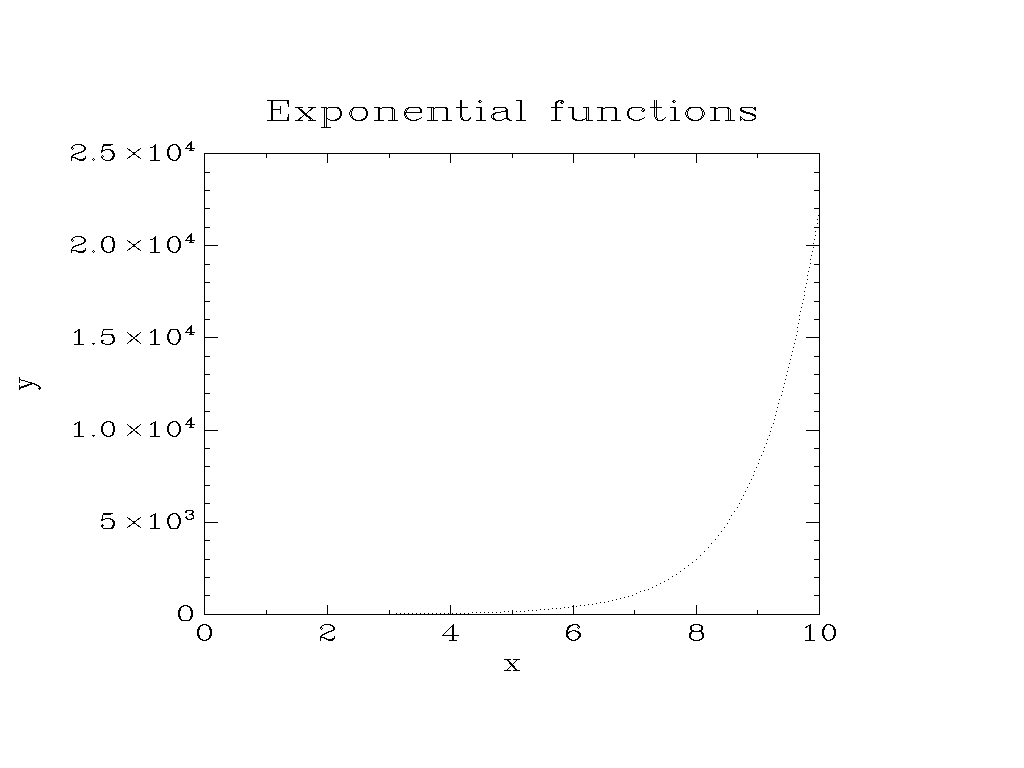
\includegraphics[scale = 0.5]{graph.png}
	\caption{Plot of the quick and dirty implementation and the built-in exponential function}
\end{figure}


\end{document}
